\documentclass[11pt, a4paper]{jsarticle}
\usepackage{multicol}  % パッケージの追加
\usepackage[dvipdfmx]{graphicx}
\begin{document}
%=============================================================
%=============================================================
\section{Polarization of Light}
\subsection*{Purpose}
この実験の目的はまずマルスの法則を確認し,S偏光とP偏光の反射において入射角ごとの反射率を測定する.またブリュースター角を測定する.
\subsection{Law of Malus}
\subsubsection{Procedure}
光学系を図\ref{fig:17}のように製作する.
今回はNDフィルターは用いなかった.
まずビーム光の光路に二つの偏光板P1,P2を挿入する.
次に偏光された光がフォトディテクターの中心に来るように調整する.
初めに二つの偏光板の偏光角をどちらも同じに揃える.
その後10°ずつP2の角度を変えていきながらフォトディテクターに検出される偏光光の強度を観測してグラフにその推移をプロットしていく.

\begin{figure}[htbp]
 \begin{center}
  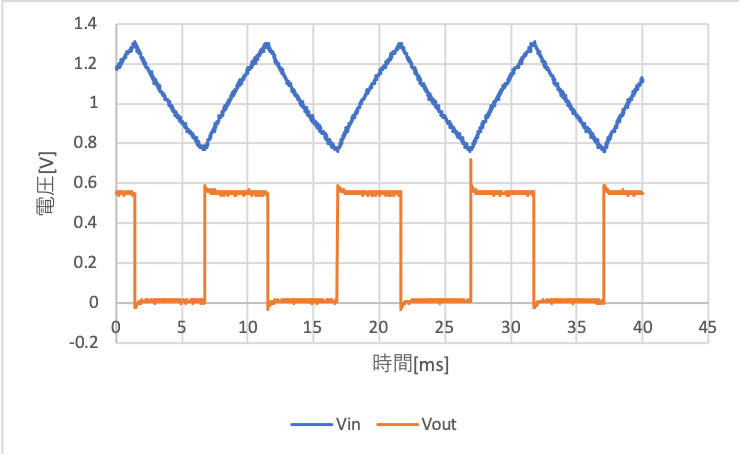
\includegraphics[width=100mm]{fig17.png}
 \end{center}
 \caption{偏光実験の光学系}
 \label{fig:17}
\end{figure}

\subsubsection{Result}
図\ref{fig:18}は実験によって得られた結果とマルスの法則によって予測される式(\ref{eq:g})をプロットしたグラフである.
ここでP1となす角を$\theta$,光の強度を$I$,偏光角0°の時の光の強度を$I_0$とした.

\begin{equation}
    I = I_0cos^2\theta \label{eq:g}
\end{equation}\\

\begin{figure}[htbp]
 \begin{center}
  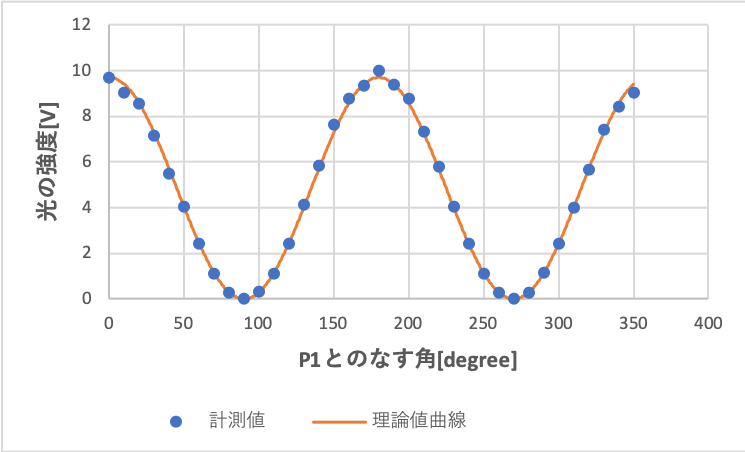
\includegraphics[width=100mm]{fig18.png}
 \end{center}
 \caption{偏光角と光の強度の強さ}
 \label{fig:18}
\end{figure}

グラフより実験での計測値とマルスの法則より導かれる式(\ref{eq:g})の結果は概ね一致した.

\subsubsection{Discussion}
グラフのように光の強度が変化したのはP1で偏光されて向きが統一されたビーム光をさらにP2で偏光するためP1,P2が垂直に近くなる程,偏光後の光の強度は小さくなっていくためであると考えられる.
また強度が$cos^2\theta$に比例する理由は,まずP2で偏光されることで波振幅はその余弦成分のみが取り出されるため,結果として強度は振幅の二乗に比例するので$cos^2\theta$に比例する結果となると考えられる.
また完全に式(\ref{eq:g})に計測結果が一致しなかったのはフォトディテクターの中心にビーム光がしっかりと当たっていなかったことが考えられる.
%=============================================================
\subsection{Reflection}
\subsubsection{Procedure}
図\ref{fig:19}のように光学系を製作する.
まず入射面に対し垂直に振幅するS偏光,入射面に対して平行に振幅するP偏光の二つの光を偏光板を使って作り出す.この時二つの偏光光の強度を等しくするためにビームの振幅は入射面に対して45°をなすように設置する.
次に偏光光をスライドガラス(屈折率 n = 1.52)に当てて反射させる.
この際スライドガラスにオイルをつけてプリズムに固定する.
その後二つの偏光光ごとに反射光の強度をフォトディテクターを用いて計測する.
反射角は10°から10°刻みに大きくしていき60°まで測定する.
特にP偏光に関してはブリュースター角付近の55°前後を2°ずつ測定する.
測定後に入射角と反射光の強度の関係をグラフにプロットする.
またブリュースター角は相対屈折率nとすれば式(\ref{eq:g})で与えられる.

\begin{equation}
    \theta_B = arctan(n) \label{eq:h}
\end{equation}\\

\begin{figure}[htbp]
 \begin{center}
  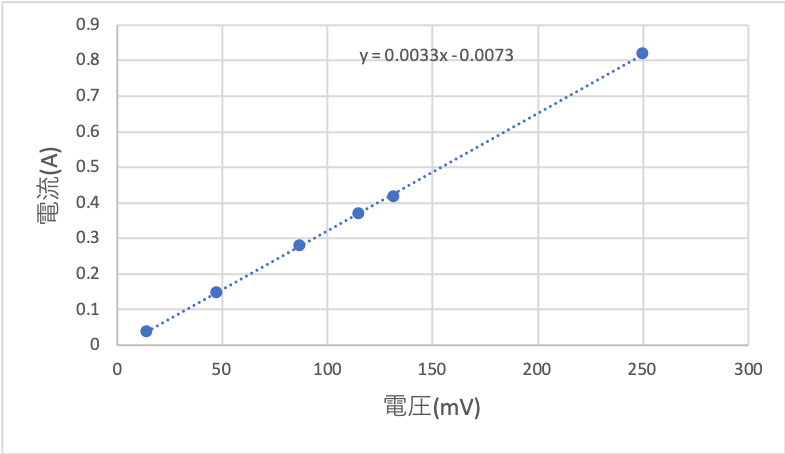
\includegraphics[width=100mm]{fig19.png}
 \end{center}
 \caption{反射強度の実験}
 \label{fig:19}
\end{figure}

\subsubsection{Result}
結果をグラフにプロットすると以下のようになった.

\begin{figure}[htbp]
 \begin{minipage}{0.45\hsize}
  \begin{center}
   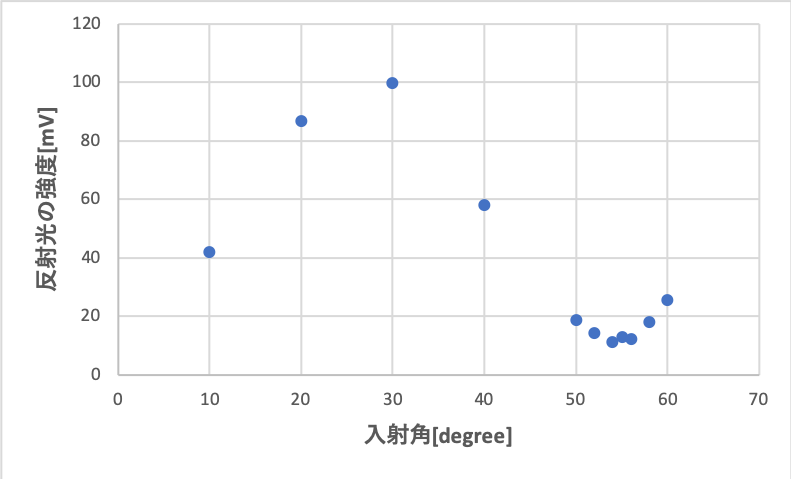
\includegraphics[width=60mm]{fig20.png}
  \end{center}
  \caption{P偏光の反射光強度}
  \label{fig:20}
 \end{minipage}
 \begin{minipage}{0.45\hsize}
  \begin{center}
   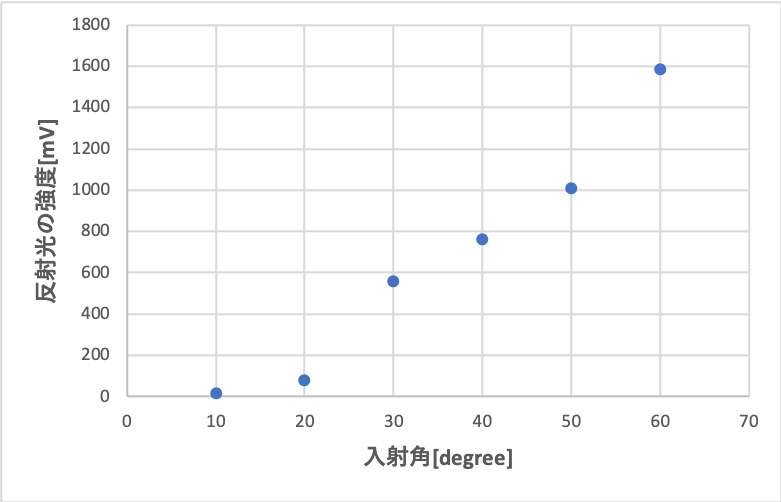
\includegraphics[width=60mm]{fig21.png}
  \end{center}
  \caption{S偏光の反射光強度}
  \label{fig:21}
 \end{minipage}
\end{figure}

グラフよりP偏光,S偏光どちらも基本的に反射角が大きくなっていくにつれて反射光の強度も強くなっていった.
またP偏光においてはブリュースター角付近で反射光の値が非常に小さくなることが確認された.
一方S偏光では反射角が大きくなるにつれて反射光強度は大きくなっていった.
またP偏光においては20°から40°において理論値のグラフ概形から大きく外れる結果となった.

\newpage
\subsubsection{Discussion}
実験からP偏光において$\theta=55°$の時に反射光の値が一番小さくなった.
つまり$\theta=55°$が実験におけるブリュースター角であると推測できる.
実際に式(\ref{eq:h})に空中の屈折率1.0,スライドガラスの屈折率1.52を考慮すると,ブリュースター角の理論値は$\theta_B=56.659$と計算でき概ね実験結果と同じ値を示した.
しかし実験において56°の値が54°,55°の値よりも大きくなり一つだけ外れた値となってしまった理由としてはフォトディテクターに反射光がまっすぐに当たらなかったことが考えられる.

また図\ref{fig:20}においてP偏光の反射強度が入射角20°から40°において理論値のグラフ概形から大きく外れてしまった原因は反射角が小さい時に光学機器同士が机上に密集していたためにフォトディテクターを安定して設置することができず中心にビーム光が当たらなかったからだと考えられる.
そのように考えると入射角が10°,20°においてP偏光の反射光強度がS偏光の反射光強度に比べて著しく低くなったことにも説明がつく.

またプリズムはスライドガラスを安定して机に固定するために用いたと考えられる.
またスライドガラスとプリズムの間にオイルを塗ったのはオイルの屈折率が1.518とガラスの屈折率に非常に近く,オイルによりプリズムとスライドガラスの間に空気を入れないためだと考えられる.
このことによってプリズムによる反射光を作り出さずにスライドガラスによって反射された光のみを測定することができるようになった働きがあると推測される.
またブリュースター角においてS偏光,P偏光の関係は図\ref{fig:25}で表される.

\begin{figure}[htbp]
 \begin{center}
  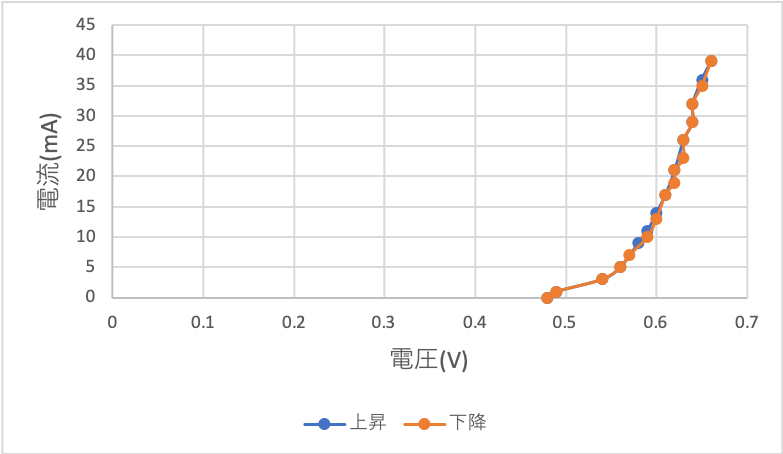
\includegraphics[width=10cm]{fig25.png}
 \end{center}
 \caption{ブリュースター角におけるS偏光P偏光の関係}
 \label{fig:25}
\end{figure}
%=============================================================
%=============================================================
\newpage
\end{document}
